%%%%%%%%%%%%%%%%%%%%%%%%%%%%%%%%%%%%%%%%%%%%%%%%%%%%%%%%%%%%%%%%%%%%%
% Template de Artigo
% XXIX ENMC – Encontro Nacional de Modelagem Computacional
% XVII ECTM – Encontro de Ciência e Tecnologia de Materiais
%%%%%%%%%%%%%%%%%%%%%%%%%%%%%%%%%%%%%%%%%%%%%%%%%%%%%%%%%%%%%%%%%%%%%

\documentclass[12pt,fleqn]{article}

%%%%%%%%%%%%%%%%%%%%%%%%%%%%%%%%%%%%%%%%%%%%%%%%%%%%%%%%%%%%%%%%%%%%%
% CONFIGURAÇÃO DE IDIOMA E CODIFICAÇÃO
%%%%%%%%%%%%%%%%%%%%%%%%%%%%%%%%%%%%%%%%%%%%%%%%%%%%%%%%%%%%%%%%%%%%%

\usepackage[utf8]{inputenc}   % Codificação UTF-8
\usepackage[T1]{fontenc}      % Codificação de fontes
\usepackage[brazil]{babel}    % Português do Brasil (Babel moderno)

%%%%%%%%%%%%%%%%%%%%%%%%%%%%%%%%%%%%%%%%%%%%%%%%%%%%%%%%%%%%%%%%%%%%%
% PACOTES DO TEMPLATE
%%%%%%%%%%%%%%%%%%%%%%%%%%%%%%%%%%%%%%%%%%%%%%%%%%%%%%%%%%%%%%%%%%%%%

\usepackage{setup/config}     % Arquivo de estilo do evento
\usepackage{natbib}           % Sistema de citações
\newcommand{\citeonline}[1]{\citet{#1}}
\usepackage{graphicx}         % Inserção de figuras
\usepackage{color}            % Controle de cores
\usepackage{wallpaper}        % Imagens de fundo
\usepackage{hyperref}         % Links e referências
\usepackage{titlesec}         % Controle de títulos
\usepackage{float}            % Permite usar [H] em figuras/tabelas
\usepackage{fancyhdr}         % Cabeçalhos e rodapés

%%%%%%%%%%%%%%%%%%%%%%%%%%%%%%%%%%%%%%%%%%%%%%%%%%%%%%%%%%%%%%%%%%%%%
% DIRETÓRIO DAS FIGURAS
%%%%%%%%%%%%%%%%%%%%%%%%%%%%%%%%%%%%%%%%%%%%%%%%%%%%%%%%%%%%%%%%%%%%%

\graphicspath{{figures/}}

%%%%%%%%%%%%%%%%%%%%%%%%%%%%%%%%%%%%%%%%%%%%%%%%%%%%%%%%%%%%%%%%%%%%%
% AJUSTE DE ESPAÇAMENTO NA BIBLIOGRAFIA
%%%%%%%%%%%%%%%%%%%%%%%%%%%%%%%%%%%%%%%%%%%%%%%%%%%%%%%%%%%%%%%%%%%%%

% Reduz espaçamento entre referências
\let\OLDthebibliography\thebibliography
\renewcommand\thebibliography[1]{%
\OLDthebibliography{#1}
\setlength{\parskip}{0pt}
\setlength{\itemsep}{0pt plus 0.3ex}
}

%%%%%%%%%%%%%%%%%%%%%%%%%%%%%%%%%%%%%%%%%%%%%%%%%%%%%%%%%%%%%%%%%%%%%
% TÍTULO DO ARTIGO
%%%%%%%%%%%%%%%%%%%%%%%%%%%%%%%%%%%%%%%%%%%%%%%%%%%%%%%%%%%%%%%%%%%%%

\title{ORDENAMENTO DE SNPs POR MÉTODOS ESTATÍSTICOS E DE APRENDIZADO DE MÁQUINA: UM ESTUDO COMPARATIVO EM BASES SIMULADAS}

%%%%%%%%%%%%%%%%%%%%%%%%%%%%%%%%%%%%%%%%%%%%%%%%%%%%%%%%%%%%%%%%%%%%%
% AUTORES E AFILIAÇÕES
%%%%%%%%%%%%%%%%%%%%%%%%%%%%%%%%%%%%%%%%%%%%%%%%%%%%%%%%%%%%%%%%%%%%%

\author{
\rm
\begin{tabular}{l}
\textbf{João Vitor Barreto Baptista}$^{1}$ - {\textnormal joaovbb@id.uff.br}\\
\textbf{Thiago Jordem Pereira}$^{1}$ - {\textnormal 
tjordem@id.uff.br}\\
\textbf{Fabrízzio Condé de Oliveira}$^{1}$ - {\textnormal 
fabrizzioconde@id.uff.br}\\
{\fontsize{11}{0}\selectfont $^{1}$Universidade Federal Fluminense - Santo Antônio de Pádua – RJ}
\end{tabular}
}

%%%%%%%%%%%%%%%%%%%%%%%%%%%%%%%%%%%%%%%%%%%%%%%%%%%%%%%%%%%%%%%%%%%%%
% RODAPÉ ESPECIAL DA PRIMEIRA PÁGINA
%%%%%%%%%%%%%%%%%%%%%%%%%%%%%%%%%%%%%%%%%%%%%%%%%%%%%%%%%%%%%%%%%%%%%

\fancypagestyle{firstpagestyle}
{
\renewcommand{\headrulewidth}{0pt}

\fancyfoot[C]{
\footnotesize
\parbox{15cm}{
\centering
\fontsize{7.5}{0}\selectfont\it
XXIX ENMC – Encontro Nacional de Modelagem Computacional\\
XVII ECTM – Encontro de Ciência e Tecnologia de Materiais\\
06 a 09 de outubro de 2026 - Bento Gonçalves - RS
}}
}

%%%%%%%%%%%%%%%%%%%%%%%%%%%%%%%%%%%%%%%%%%%%%%%%%%%%%%%%%%%%%%%%%%%%%
% INÍCIO DO DOCUMENTO
%%%%%%%%%%%%%%%%%%%%%%%%%%%%%%%%%%%%%%%%%%%%%%%%%%%%%%%%%%%%%%%%%%%%%

\begin{document}

\pretolerance=10000

%%%%%%%%%%%%%%%%%%%%%%%%%%%%%%%%%%%%%%%%%%%%%%%%%%%%%%%%%%%%%%%%%%%%%
% LOGO DO EVENTO
%%%%%%%%%%%%%%%%%%%%%%%%%%%%%%%%%%%%%%%%%%%%%%%%%%%%%%%%%%%%%%%%%%%%%

\begin{figure}
\centering

\includegraphics[width=6.25in]{logo.png}
\end{figure}

\vspace{-3cm}

%%%%%%%%%%%%%%%%%%%%%%%%%%%%%%%%%%%%%%%%%%%%%%%%%%%%%%%%%%%%%%%%%%%%%
% TÍTULO
%%%%%%%%%%%%%%%%%%%%%%%%%%%%%%%%%%%%%%%%%%%%%%%%%%%%%%%%%%%%%%%%%%%%%

\maketitle

\pagestyle{empty}
\thispagestyle{firstpagestyle}

%%%%%%%%%%%%%%%%%%%%%%%%%%%%%%%%%%%%%%%%%%%%%%%%%%%%%%%%%%%%%%%%%%%%%
% RESUMO
%%%%%%%%%%%%%%%%%%%%%%%%%%%%%%%%%%%%%%%%%%%%%%%%%%%%%%%%%%%%%%%%%%%%%

\begin{abstract}
A seleção de marcadores genéticos relevantes é uma etapa central em estudos de associação genômica ampla (GWAS). Neste trabalho, seis métodos de ordenamento de \emph{Single Nucleotide Polymorphisms} (SNPs) são comparados em duas bases de dados simuladas: a primeira com oito efeitos genéticos independentes e a segunda com efeitos marginais combinados a interações epistáticas em par e em trio. Os métodos avaliados são Correlação Marginal, Correlação Parcial, CAR Score, I Score, Importância por Permutação e Importância por Impureza, sendo os dois últimos extraídos de uma mesma Random Forest. Os resultados mostram que, no cenário de efeitos independentes, a maioria dos métodos recupera os SNPs causais entre as primeiras posições. Na presença de interações epistáticas, o desempenho se deteriora, especialmente para SNPs sem efeito marginal direto: a Importância por Permutação foi o único método capaz de posicionar o SNP envolvido exclusivamente na interação tripla entre os 15 primeiros. Nenhum método se mostrou superior em todos os cenários, indicando complementariedade entre as abordagens.
\end{abstract}

\keywords{\em{Aprendizado de Máquinas, GWAS, Métodos de ordenamentos, SNPs.}}

%%%%%%%%%%%%%%%%%%%%%%%%%%%%%%%%%%%%%%%%%%%%%%%%%%%%%%%%%%%%%%%%%%%%%
% CABEÇALHO DAS DEMAIS PÁGINAS
%%%%%%%%%%%%%%%%%%%%%%%%%%%%%%%%%%%%%%%%%%%%%%%%%%%%%%%%%%%%%%%%%%%%%

\fancyhead[L]{\footnotesize{\fontsize{7.5}{0}\selectfont\it
XXIX ENMC, XVII ECTM\\
06 a 09 de outubro de 2026}}

\renewcommand{\headrulewidth}{0pt}

\fancyfoot[C]{
\footnotesize
\parbox{15cm}{
\centering
\fontsize{7.5}{0}\selectfont\it
XXIX ENMC – Encontro Nacional de Modelagem Computacional\\
XVII ECTM – Encontro de Ciência e Tecnologia de Materiais\\
06 a 09 de outubro de 2026 - Bento Gonçalves - RS
}}

\rhead{}

\pagestyle{fancy}

%%%%%%%%%%%%%%%%%%%%%%%%%%%%%%%%%%%%%%%%%%%%%%%%%%%%%%%%%%%%%%%%%%%%%
% INÍCIO DO TEXTO
%%%%%%%%%%%%%%%%%%%%%%%%%%%%%%%%%%%%%%%%%%%%%%%%%%%%%%%%%%%%%%%%%%%%%

\section{INTRODUÇÃO}

A identificação de variáveis relevantes é uma etapa fundamental em estudos de associação genômica ampla, conhecidos como GWAS (\emph{Genome-Wide Association Studies}). Nesses estudos, o elevado número de variáveis explicativas, aliado à presença de correlações entre marcadores genéticos e de possíveis relações complexas com o fenótipo de interesse, torna a seleção de preditores um problema estatístico e computacional desafiador. Por essa razão, diferentes métodos têm sido propostos para estabelecer critérios de ordenamento capazes de identificar as variáveis mais relevantes.

Neste trabalho são empregados seis métodos de ordenamento de variáveis com o objetivo de avaliar diferentes estratégias para identificar \emph{Single Nucleotide Polymorphisms} (\emph{SNPs}) potencialmente associados ao fenótipo de interesse. Essas abordagens diferem quanto ao critério utilizado para mensurar a relevância das variáveis, abrangendo desde medidas baseadas em associação linear até métodos capazes de considerar estruturas de dependência entre os preditores ou relações não lineares. A comparação entre esses métodos busca analisar como diferentes critérios de ordenamento influenciam a priorização dos marcadores genéticos.

É importante ressaltar que o ordenamento dos \emph{SNPs}, por si só, não determina quais marcadores devem ser selecionados como relevantes. Para isso, é necessário associar ao \emph{ranking} um critério de corte que estabeleça um limiar de seleção. O critério mais difundido em estudos de associação genômica consiste em reter os \emph{SNPs} cujo valor-p é inferior ou igual a $0{,}05$. Entretanto, outros métodos têm sido propostos na literatura, como o SMS (\emph{SNP Markers Selector}), apresentado por \citeonline{Oliveira2015}, que estrutura o processo de seleção em três etapas: (i) ordenamento dos marcadores pela importância obtida por uma \emph{Random Forest}; (ii) corte automático, no qual subconjuntos crescentes de \emph{SNPs}, definidos a partir do \emph{ranking}, são avaliados por um SVM/SVR e o subconjunto com melhor desempenho preditivo é selecionado; e (iii) refinamento, em que um Algoritmo Genético busca a melhor combinação de marcadores dentre os selecionados na etapa anterior, com o objetivo de identificar \emph{SNPs} verdadeiros positivos e eliminar falsos-positivos. A investigação de critérios de corte, contudo, foge ao escopo deste trabalho, que se concentra exclusivamente na comparação dos métodos de ordenamento.

Os métodos investigados são: Correlação Marginal, Correlação Parcial, \emph{CAR Score}, \emph{I Score}, Importância por Permutação (\emph{Permutation Importance}) e Importância por Impureza (\emph{Mean Decrease Impurity}), sendo estes dois últimos obtidos a partir de uma mesma \emph{Random Forest}. Cada um deles adota uma estratégia distinta para avaliar a contribuição das variáveis em relação ao fenótipo analisado. Nas subseções seguintes, esses métodos são apresentados de forma sucinta, destacando seus principais fundamentos e critérios de ordenamento.

\section{MÉTODOS DE ORDENAMENTO DE VARIÁVEIS}

Nesta seção são apresentados os métodos de ordenamento de variáveis considerados neste estudo, os quais foram utilizados para ranquear os \emph{SNPs} de acordo com sua relevância para o fenótipo analisado. A seguir, apresenta-se uma breve descrição de cada um deles.

\subsection{Correlação Marginal}

A correlação marginal avalia a associação linear entre uma variável explicativa \(X_i\) e a variável resposta \(Y\), sendo calculada por

\begin{equation}
\rho_{X_{i}Y} = \frac{\text{Cov}(X_i, Y)}{\sigma_{X_i}\sigma_Y},
\end{equation}

\noindent em que $\text{Cov}(X_i,Y)$ é a covariância entre $X_i$ e $Y$, $\sigma_{X_i}$ é o desvio-padrão de $X_i$ e $\sigma_Y$ é o desvio-padrão de $Y$.

A ordenação dos \emph{SNPs} pelo valor absoluto da correlação marginal é equivalente à ordenação pelo valor-p da regressão linear simples entre cada \emph{SNP} e o fenótipo~\citep{moretin2023, FanLv2008}. Essa equivalência decorre do fato de a estatística $t$ do teste de significância do coeficiente angular ser uma transformação monotônica do coeficiente de correlação amostral, conforme demonstrado a seguir.

Considere o modelo de regressão linear simples $Y = \beta_0 + \beta_1 X_i + \varepsilon$, em que $\varepsilon \sim N(0, \sigma^2)$. O estimador de mínimos quadrados ordinários do coeficiente angular é $\hat{\beta}_1 = \text{Cov}(X_i, Y) / \text{Var}(X_i)$, e a estatística $t$ para testar $H_0\!: \beta_1 = 0$ contra $H_1\!: \beta_1 \neq 0$ pode ser escrita como

\begin{equation}
t = r_{X_iY} \sqrt{\frac{n-2}{1 - r_{X_iY}^2}},
\label{eq:t_corr}
\end{equation}

\noindent em que $r_{X_iY}$ é o coeficiente de correlação amostral de Pearson entre $X_i$ e $Y$ e $n$ é o número de observações. A Equação~\ref{eq:t_corr} mostra que $|t|$ é uma função exclusivamente de $|r_{X_iY}|$ (para $n$ fixo). Além disso, a função $g(r) = |r|\sqrt{(n-2)/(1-r^2)}$ é estritamente crescente em $|r|$ no intervalo $[0,1)$, pois sua derivada em relação a $|r|$ é positiva nesse domínio. Portanto,

\begin{equation}
|r_{X_iY}| > |r_{X_jY}| \;\Longleftrightarrow\; |t_i| > |t_j| \;\Longleftrightarrow\; p_i < p_j,
\label{eq:equivalencia}
\end{equation}

\noindent em que $p_i$ e $p_j$ são os valores-p bicaudais associados a $t_i$ e $t_j$, respectivamente (a última equivalência segue do fato de a distribuição $t$ de Student ser simétrica e unimodal). Assim, ordenar os \emph{SNPs} por $|r_{X_iY}|$ decrescente produz exatamente o mesmo \emph{ranking} que ordená-los por valor-p crescente, razão pela qual ambos os critérios foram tratados como um único método neste estudo.

\subsection{Correlação Parcial}

O segundo método considerado neste trabalho é a correlação parcial, que quantifica a associação linear entre uma variável explicativa e a variável resposta após remover o efeito linear das demais variáveis explicativas. No caso de duas variáveis explicativas, essa medida é definida por

\begin{equation}
\rho_{Y, X_1 | X_2} =
\frac{\rho_{YX_1} - \rho_{YX_2}\rho_{X_{1}X_{2}}}
{\sqrt{(1-\rho_{YX_2}^2)(1-\rho_{X_{1}X_{2}}^2)}},
\end{equation}

\noindent em que $\rho_{Y,X_1|X_2}$ representa a correlação parcial entre $Y$ e $X_1$ condicionada a $X_2$, $\rho_{YX_1}$ e $\rho_{YX_2}$ são as correlações marginais entre $Y$ e as variáveis $X_1$ e $X_2$, respectivamente, e $\rho_{X_1X_2}$ é a correlação entre as variáveis explicativas. No caso geral com $p$ variáveis, a correlação parcial entre $Y$ e $X_i$ condicionada às $p-1$ variáveis restantes é obtida a partir da inversa da matriz de correlação, conforme o estimador com \emph{shrinkage} proposto por \citeonline{schafer2005}.

\subsection{CAR Score}

O \textit{CAR Score} (\textit{Correlation-Adjusted Score}) é um método de ordenamento de variáveis empregado em modelos de regressão linear, que ajusta as correlações marginais de acordo com a dependência existente entre os preditores. Sua definição é dada por

\begin{equation}
\omega = P^{-1/2}P_{XY},
\end{equation}

\noindent em que $P$ é a matriz de correlação das variáveis explicativas e $P_{XY}$ é o vetor de correlações marginais entre as variáveis explicativas e a variável resposta.

\cite{ZuberStrimmer2011}

\subsection{I Score}

O \textit{I Score} (\textit{Importance Score}) é um método de ordenamento de variáveis que quantifica a contribuição de cada preditor para a variação da variável resposta, sendo definido por

\begin{equation}
    I=\sum_{j=1}^{m_1} \frac{n_j}{n} \frac{(\overline{Y_j}-\overline{Y})^2}{s^2/n_j} =
    \frac{\sum_{j=1}^{m_1} n_j^2 (\overline{Y_j}-\overline{Y})^2}
    {\sum_{i=1}^{n}(Y_i-\overline{Y})^2}.
\end{equation}

\noindent em que $\overline{Y}$ representa a média da variável resposta, $\overline{Y_j}$ é a média da resposta para a $j$-ésima categoria da variável explicativa, $n_j$ é o número de observações nessa categoria, $n$ é o número total de observações e $s^2$ é a variância da variável resposta.

\cite{Lo2015}

\subsection{Importância por Permutação (Permutation Importance)}

A Importância por Permutação, também conhecida como \textit{Permutation Importance}, quantifica a contribuição de uma variável explicativa a partir do aumento do erro de predição de uma \textit{Random Forest} quando os valores dessa variável são aleatoriamente permutados entre as observações \textit{out-of-bag} (OOB) de cada árvore. Diferentemente da Importância por Impureza, esse método avalia a variável em relação à sua capacidade preditiva efetiva, e não apenas à frequência e à qualidade das divisões em que ela é utilizada. A importância da variável $X_j$ é dada por

\begin{equation}
    \text{VI}(X_j) = \frac{1}{B} \sum_{b=1}^{B} \left[ \frac{1}{|OOB_b|} \sum_{i \in OOB_b} \left(y_i - \hat{y}_i^{(b,\pi_j)}\right)^2 - \frac{1}{|OOB_b|} \sum_{i \in OOB_b} \left(y_i - \hat{y}_i^{(b)}\right)^2 \right],
\end{equation}

\noindent em que $B$ é o número de árvores da floresta, $OOB_b$ é o conjunto de observações \textit{out-of-bag} da árvore $T_b$ (isto é, as observações não utilizadas no ajuste de $T_b$), $y_i$ é o valor observado do fenótipo, $\hat{y}_i^{(b)}$ é o valor predito para a observação $i$ pela árvore $T_b$ e $\hat{y}_i^{(b,\pi_j)}$ é o valor predito para a mesma observação após a permutação aleatória dos valores de $X_j$ entre as observações de $OOB_b$.

Quanto maior o aumento do erro de predição após a permutação de uma variável, maior é sua relevância para o processo preditivo. Dessa forma, o método é capaz de identificar variáveis importantes mesmo na presença de relações não lineares e interações entre preditores.

\citep{breiman2001random, Strobl2007, Strobl2008}

\subsection{Importância por Impureza (Mean Decrease Impurity)}

A Importância por Impureza, também conhecida como \textit{Mean Decrease Impurity} (MDI), quantifica a contribuição de uma variável explicativa a partir da redução de impureza que ela proporciona ao longo das divisões (\textit{splits}) de uma \textit{Random Forest}. Como o fenótipo considerado neste estudo é contínuo, a impureza de um nó $t$ é medida pela soma de quadrados dos resíduos (RSS) em torno da média do nó, e não pelo índice de Gini — este último aplicável apenas a variáveis resposta categóricas. A importância da variável $X_j$ é dada por

\begin{equation}
    \text{Imp}(X_j) = \frac{1}{B} \sum_{b=1}^{B} \sum_{t \in T_b:\, v(t) = X_j} p(t)\, \Delta i(t),
\end{equation}

\noindent em que $B$ é o número de árvores da floresta, a soma interna percorre todos os nós $t$ da árvore $T_b$ em que a divisão utiliza a variável $X_j$, $p(t) = n_t/n$ é a proporção de observações que alcançam o nó $t$ e $\Delta i(t)$ é o decréscimo de impureza promovido pela divisão, definido por

\begin{equation}
    \Delta i(t) = RSS(t) - \left[ \frac{n_{tL}}{n_t} RSS(t_L) + \frac{n_{tR}}{n_t} RSS(t_R) \right],
\end{equation}

\noindent em que $t_L$ e $t_R$ são os nós filhos esquerdo e direito gerados pela divisão de $t$.

\citep{breiman2001random, Scornet2023}

As duas medidas descritas nesta e na subseção anterior são extraídas de uma única \textit{Random Forest} ajustada para cada base de dados com a função \texttt{randomForest} do pacote homônimo do R, utilizando $B = 4\,000$ árvores, $mtry = \lfloor p/3 \rfloor$ e os demais hiperparâmetros em seus valores padrão (\texttt{nodesize} $= 5$, \texttt{replace = TRUE}, \texttt{sampsize} $= n$). A Importância por Permutação corresponde ao \texttt{\%IncMSE} e a Importância por Impureza ao \texttt{IncNodePurity}. Uma semente fixa (\texttt{seed = 123}) foi utilizada em todas as etapas, garantindo a reprodutibilidade dos resultados. Todas as análises computacionais deste estudo foram realizadas no ambiente estatístico R~\citep{R}.

\subsection{Natureza determinística e estocástica dos métodos}

Dos seis métodos considerados, quatro são determinísticos --- Correlação Marginal, Correlação Parcial, CAR Score e I Score --- pois dependem exclusivamente de quantidades amostrais fixas, produzindo sempre o mesmo ordenamento para uma mesma base de dados. Por outro lado, a Importância por Permutação e a Importância por Impureza são estocásticas, pois dependem da \textit{Random Forest}, cujo ajuste envolve reamostragem \textit{bootstrap} e seleção aleatória de variáveis candidatas em cada divisão; a Importância por Permutação acrescenta ainda o embaralhamento dos valores nas observações \textit{out-of-bag}. Assim, a alteração da semente (\texttt{seed}), do número de árvores ($B$), de $mtry$ ou do \texttt{sampsize} pode produzir ordenamentos distintos.

\section{BASE DE DADOS SIMULADA}

Foram simuladas duas bases de dados com o objetivo de comparar o desempenho dos métodos de ordenamento em cenários de complexidade distinta. Os desenhos reproduzem a Simulação~1 e a Simulação~4 descritas na tese de doutorado de \citeonline{Oliveira2015}: a Base de Dados~1 corresponde à Simulação~1, com oito efeitos genéticos independentes e sem interações epistáticas; a Base de Dados~2 corresponde à Simulação~4, com três efeitos marginais isolados, uma interação epistática em par e uma interação em trio. Ambas as bases são geradas com fenótipo contínuo por meio do modelo linear generalizado para SNPs implementado na função \texttt{simulateSNPglm} do pacote \texttt{scrime} do R \citep{Schwender2013}, que considera a codificação $1$ para homozigotos de referência \textit{AA}, $2$ para heterozigotos \textit{Aa} e $3$ para homozigotos variantes \textit{aa}. Cada base possui $n = 1\,000$ indivíduos e $p = 100$ \emph{SNPs}, dos quais apenas os marcados como causais contribuem para a formação do fenótipo.

Em ambas as bases, o fenótipo contínuo $y$ é gerado pelo modelo linear descrito pelas Equações \ref{eq:base1} e \ref{eq:base2}, em que cada $L_k$ é uma variável indicadora (igual a $1$ quando a condição genotípica associada é satisfeita, e $0$ caso contrário), o operador $\mathbin{\&}$ denota a ocorrência simultânea das condições envolvidas em interações epistáticas, e \emph{erro} é uma variável aleatória normal com média zero e desvio padrão igual a um.

\subsection{Base de Dados 1 --- Oito Efeitos Independentes (Simulação~1)}

Este primeiro cenário reproduz a Simulação~1 de \citeonline{Oliveira2015}, com oito \emph{SNPs} causais ($SNP1$ a $SNP8$), cada um com efeito independente sobre o fenótipo (sem interações epistáticas). O modelo utilizado é apresentado na Equação \ref{eq:base1}.

\begin{equation}
    y = \beta_0 + \beta_1 L_1 + \beta_2 L_2 + \beta_3 L_3 + \beta_4 L_4 + \beta_5 L_5 + \beta_6 L_6 + \beta_7 L_7 + \beta_8 L_8 + \text{erro},
    \label{eq:base1}
\end{equation}

\noindent em que \emph{erro} $\sim N(0,1)$ e as variáveis explicativas são definidas por
$L_1 = (SNP1 = 1)$, $L_2 = (SNP2 = 2)$, $L_3 = (SNP3 = 3)$, $L_4 = (SNP4 \neq 1)$, $L_5 = (SNP5 \neq 2)$, $L_6 = (SNP6 \neq 3)$, $L_7 = (SNP7 = 1)$ e $L_8 = (SNP8 = 2)$. A expressão $(SNPj = k)$ indica que o efeito do $SNPj$ é destacado quando o genótipo desse marcador é igual a $k$ (sendo $1$ o homozigoto de referência \textit{AA}, $2$ o heterozigoto \textit{Aa} e $3$ o homozigoto variante \textit{aa}); analogamente, $(SNPj \neq k)$ indica que o efeito é destacado quando o genótipo é diferente de $k$. Para os coeficientes, adotou-se $\beta_0 = 640$ e $\beta_k = 1$ para $k = 1, \dots, 8$.

Nas Figuras \ref{fig:histograma1} e \ref{fig:grafico1}, observa-se a distribuição do fenótipo simulado neste cenário de efeitos independentes.

\begin{figure}[H]
    \centering
    \begin{minipage}{0.48\textwidth}
        \centering
        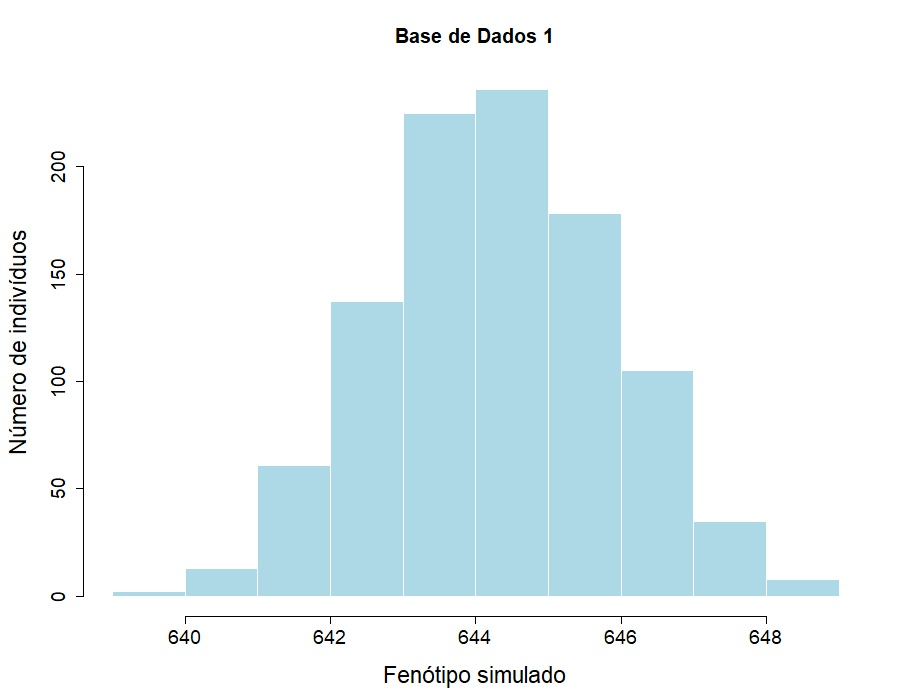
\includegraphics[width=\textwidth]{figures/histograma_base1.jpeg}
        \caption{Histograma do fenótipo simulado na Base de Dados 1.}
        \label{fig:histograma1}
    \end{minipage}
    \hfill
    \begin{minipage}{0.48\textwidth}
        \centering
        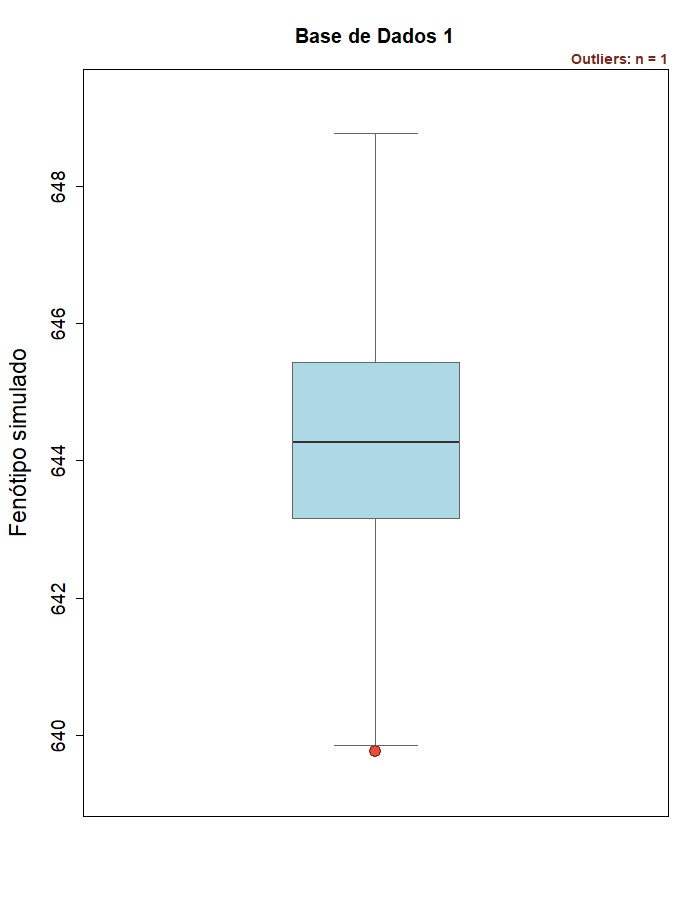
\includegraphics[width=\textwidth]{figures/boxplot_base1.jpeg}
        \caption{Boxplot do fenótipo simulado na Base de Dados 1.}
        \label{fig:grafico1}
    \end{minipage}
\end{figure}

\subsection{Base de Dados 2 --- Três Efeitos Marginais, uma Interação em Par e uma Interação em Trio (Simulação~4)}

O segundo cenário reproduz a Simulação~4 de \citeonline{Oliveira2015}, com três efeitos marginais isolados ($SNP1$, $SNP2$ e $SNP3$) e duas interações epistáticas envolvendo, respectivamente, o par ($SNP4$, $SNP5$) e o trio ($SNP6$, $SNP7$, $SNP8$). O modelo completo, na mesma notação da Equação \ref{eq:base1}, é apresentado na Equação \ref{eq:base2}.

\begin{equation}
    y = \beta_0 + \beta_1 L_1 + \beta_2 L_2 + \beta_3 L_3 + \beta_4 L_4 + \beta_5 L_5 + \text{erro},
    \label{eq:base2}
\end{equation}

\noindent em que \emph{erro} $\sim N(0,1)$ e as variáveis explicativas são definidas por
$L_1 = (SNP1 = 1)$, $L_2 = (SNP2 = 2)$, $L_3 = (SNP3 = 3)$, $L_4 = (SNP4 \neq 1) \mathbin{\&} (SNP5 = 3)$ e $L_5 = (SNP6 = 1) \mathbin{\&} (SNP7 = 2) \mathbin{\&} (SNP8 = 3)$. As expressões $L_4$ e $L_5$ representam, respectivamente, a interação epistática em par entre os \emph{SNPs} $4$ e $5$ e a interação tripla entre os \emph{SNPs} $6$, $7$ e $8$. Para os coeficientes, adotou-se $\beta_0 = 640$, $\beta_1 = 2$, $\beta_2 = 1{,}3$, $\beta_3 = 0{,}9$, $\beta_4 = 2$ e $\beta_5 = 3$. Os oito \emph{SNPs} causais desta base são $SNP1, \dots, SNP8$. Esse desenho permite avaliar se os métodos conseguem identificar \emph{SNPs} cujo efeito se manifesta apenas por meio de interações epistáticas.

Nas Figuras \ref{fig:histograma2} e \ref{fig:grafico2}, observa-se a distribuição do fenótipo simulado neste cenário com efeitos mistos.

\begin{figure}[H]
    \centering
    \begin{minipage}{0.48\textwidth}
        \centering
        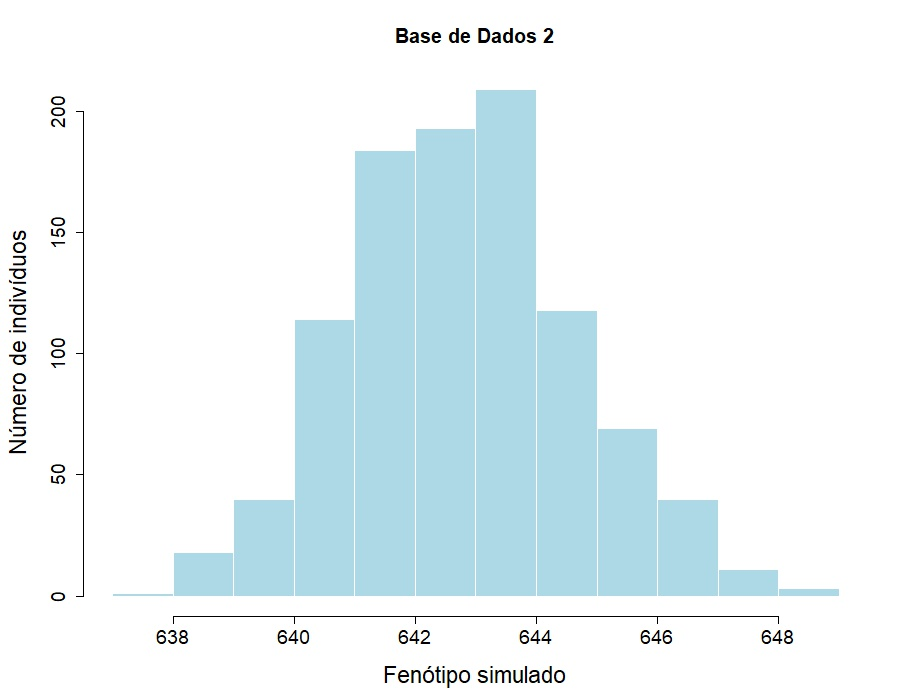
\includegraphics[width=\textwidth]{figures/histograma_base2.jpeg}
        \caption{Histograma do fenótipo simulado na Base de Dados 2.}
        \label{fig:histograma2}
    \end{minipage}
    \hfill
    \begin{minipage}{0.48\textwidth}
        \centering
        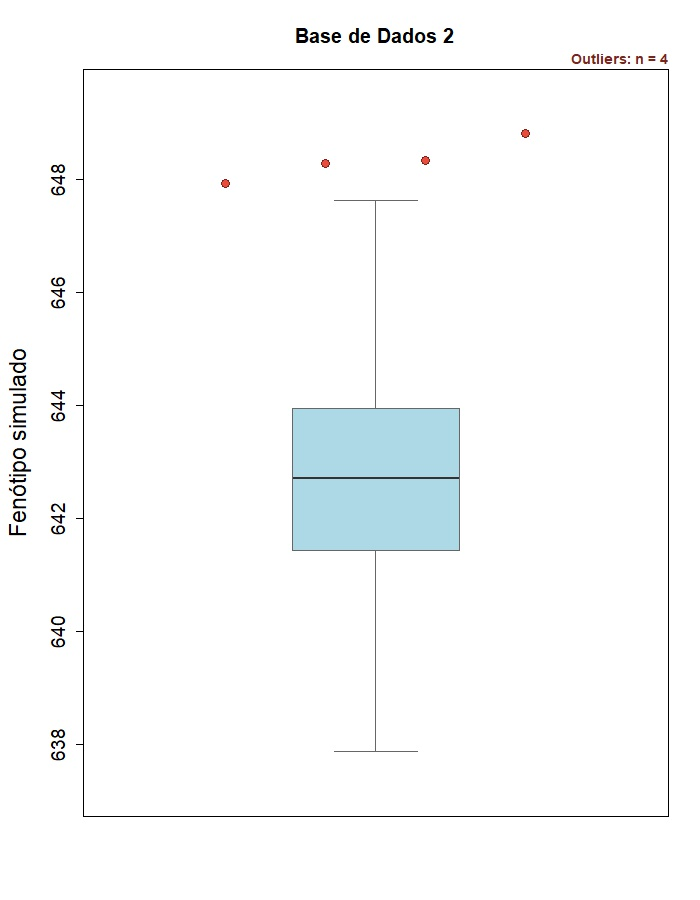
\includegraphics[width=\textwidth]{figures/boxplot_base2.jpeg}
        \caption{Boxplot do fenótipo simulado na Base de Dados 2.}
        \label{fig:grafico2}
    \end{minipage}
\end{figure}


\section{RESULTADOS NUMÉRICOS}

\subsection{Base de Dados 1}

Na Tabela \ref{tab 33} são apresentados os 15 primeiros \emph{SNPs} ranqueados por seis métodos de ordenamento na Base de Dados 1 (Simulação~1), com oito efeitos genéticos independentes ($SNP1$ a $SNP8$).

\begin{table}[H]
\centering
\caption{Rank dos SNPs por seis métodos de ordenamento para os 15 primeiros SNPs na Base de Dados 1.}
\label{tab 33}
\footnotesize
\begin{tabular}{l|l|l|l|l|l}
  \hline
\begin{tabular}[c]{@{}c@{}}Correlação\\Marginal\end{tabular} & \begin{tabular}[c]{@{}c@{}}Correlação\\Parcial\end{tabular} & CAR Score & I Score & \begin{tabular}[c]{@{}c@{}}Importância\\por Permutação\end{tabular} & \begin{tabular}[c]{@{}c@{}}Importância\\por Impureza\end{tabular} \\
  \hline
  \textbf{SNP1} & \textbf{SNP7} & \textbf{SNP7} & \textbf{SNP5} & \textbf{SNP7} & \textbf{SNP1} \\
  \textbf{SNP7} & \textbf{SNP1} & \textbf{SNP1} & \textbf{SNP1} & \textbf{SNP1} & \textbf{SNP7} \\
  \textbf{SNP4} & \textbf{SNP4} & \textbf{SNP4} & \textbf{SNP8} & \textbf{SNP4} & \textbf{SNP5} \\
  \textbf{SNP8} & \textbf{SNP5} & \textbf{SNP8} & \textbf{SNP7} & \textbf{SNP8} & \textbf{SNP4} \\
  \textbf{SNP5} & \textbf{SNP8} & \textbf{SNP5} & \textbf{SNP2} & \textbf{SNP5} & \textbf{SNP8} \\
  \textbf{SNP2} & \textbf{SNP2} & \textbf{SNP2} & \textbf{SNP4} & \textbf{SNP2} & \textbf{SNP2} \\
  SNP10 & SNP68 & SNP10 & SNP68 & \textbf{SNP3} & SNP69 \\
  SNP60 & SNP36 & SNP60 & SNP60 & SNP71 & \textbf{SNP3} \\
  SNP12 & SNP83 & SNP12 & \textbf{SNP6} & SNP51 & SNP12 \\
  SNP71 & SNP10 & SNP88 & SNP82 & SNP83 & SNP71 \\
  \textbf{SNP6} & SNP60 & SNP68 & SNP10 & SNP36 & SNP20 \\
  SNP88 & SNP88 & SNP83 & SNP58 & SNP10 & SNP68 \\
  \textbf{SNP3} & SNP56 & SNP71 & SNP20 & SNP27 & SNP11 \\
  SNP83 & SNP51 & \textbf{SNP3} & SNP89 & SNP94 & SNP10 \\
  SNP82 & \textbf{SNP3} & SNP51 & SNP36 & SNP11 & SNP89 \\
   \hline
\end{tabular}
\end{table}

Na Tabela \ref{tab 33}, os oito \emph{SNPs} causais aparecem entre os 15 primeiros em praticamente todos os métodos. Destacam-se $SNP1$ e $SNP7$, que ocupam posições elevadas de forma consistente. Já o $SNP6$, associado ao modelo recessivo reverso, apresenta ranks mais baixos na Correlação Parcial (37º) e na Importância por Impureza (85º), embora seja recuperado pelo I Score (9º) e pela Correlação Marginal (11º), conforme a Tabela \ref{tab 34}.

\begin{table}[H]
\centering
\caption{Posição dos SNPs causais por seis métodos de ordenamento na Base de Dados 1.}
\label{tab 34}
\small
\begin{tabular}{l|r|r|r|r|r|r}
  \hline
SNPs & \begin{tabular}[c]{@{}c@{}}Correlação\\Marginal\end{tabular} & \begin{tabular}[c]{@{}c@{}}Correlação\\Parcial\end{tabular} & CAR Score & I Score & \begin{tabular}[c]{@{}c@{}}Importância\\por Permutação\end{tabular} & \begin{tabular}[c]{@{}c@{}}Importância\\por Impureza\end{tabular} \\
  \hline
  SNP1 & 1º & 2º & 2º & 2º & 2º & 1º \\
  SNP2 & 6º & 6º & 6º & 5º & 6º & 6º \\
  SNP3 & 13º & 15º & 14º & 27º & 7º & 8º \\
  SNP4 & 3º & 3º & 3º & 6º & 3º & 4º \\
  SNP5 & 5º & 4º & 5º & 1º & 5º & 3º \\
  SNP6 & 11º & 37º & 18º & 9º & 36º & 85º \\
  SNP7 & 2º & 1º & 1º & 4º & 1º & 2º \\
  SNP8 & 4º & 5º & 4º & 3º & 4º & 5º \\
   \hline
\end{tabular}
\end{table}

\subsection{Base de Dados 2}

Na Tabela \ref{tab 35} são apresentados os 15 primeiros \emph{SNPs} ranqueados por seis métodos de ordenamento na Base de Dados 2, que combina três efeitos marginais, uma interação em par ($SNP4$ e $SNP5$) e uma interação em trio ($SNP6$, $SNP7$ e $SNP8$).

\begin{table}[H]
\centering
\caption{Rank dos SNPs por seis métodos de ordenamento para os 15 primeiros SNPs na Base de Dados 2.}
\label{tab 35}
\footnotesize
\begin{tabular}{l|l|l|l|l|l}
  \hline
\begin{tabular}[c]{@{}c@{}}Correlação\\Marginal\end{tabular} & \begin{tabular}[c]{@{}c@{}}Correlação\\Parcial\end{tabular} & CAR Score & I Score & \begin{tabular}[c]{@{}c@{}}Importância\\por Permutação\end{tabular} & \begin{tabular}[c]{@{}c@{}}Importância\\por Impureza\end{tabular} \\
  \hline
  \textbf{SNP1} & \textbf{SNP1} & \textbf{SNP1} & \textbf{SNP1} & \textbf{SNP1} & \textbf{SNP1} \\
  \textbf{SNP4} & \textbf{SNP4} & \textbf{SNP4} & \textbf{SNP2} & \textbf{SNP4} & \textbf{SNP5} \\
  \textbf{SNP8} & \textbf{SNP2} & \textbf{SNP2} & \textbf{SNP4} & \textbf{SNP5} & \textbf{SNP4} \\
  \textbf{SNP2} & \textbf{SNP8} & \textbf{SNP8} & \textbf{SNP5} & \textbf{SNP2} & \textbf{SNP2} \\
  \textbf{SNP5} & \textbf{SNP5} & \textbf{SNP5} & \textbf{SNP8} & \textbf{SNP8} & \textbf{SNP8} \\
  SNP10 & SNP44 & SNP10 & \textbf{SNP7} & \textbf{SNP7} & \textbf{SNP7} \\
  SNP44 & SNP68 & SNP44 & SNP17 & \textbf{SNP3} & \textbf{SNP3} \\
  SNP15 & SNP10 & \textbf{SNP3} & SNP10 & \textbf{SNP6} & SNP10 \\
  \textbf{SNP3} & \textbf{SNP7} & SNP15 & SNP43 & SNP10 & SNP89 \\
  SNP11 & SNP83 & SNP83 & SNP83 & SNP41 & SNP68 \\
  SNP17 & SNP36 & SNP11 & SNP89 & SNP91 & SNP12 \\
  SNP32 & SNP53 & SNP68 & SNP15 & SNP46 & SNP31 \\
  SNP96 & SNP75 & SNP17 & SNP96 & SNP18 & SNP69 \\
  SNP91 & SNP93 & SNP91 & SNP44 & SNP83 & SNP59 \\
  SNP39 & \textbf{SNP3} & \textbf{SNP7} & SNP88 & SNP89 & SNP87 \\
   \hline
\end{tabular}
\end{table}

Na Tabela \ref{tab 35}, o $SNP6$ --- componente da interação tripla cujo efeito marginal é nulo --- aparece apenas entre os 15 primeiros no rank da Importância por Permutação. Nos demais métodos, ele não é capturado nesse recorte, evidenciando a dificuldade de identificar \emph{SNPs} envolvidos exclusivamente em interações de ordem superior.

\begin{table}[H]
\centering
\caption{Posição dos SNPs causais por seis métodos de ordenamento na Base de Dados 2.}
\label{tab 36}
\small
\begin{tabular}{l|r|r|r|r|r|r}
  \hline
SNPs & \begin{tabular}[c]{@{}c@{}}Correlação\\Marginal\end{tabular} & \begin{tabular}[c]{@{}c@{}}Correlação\\Parcial\end{tabular} & CAR Score & I Score & \begin{tabular}[c]{@{}c@{}}Importância\\por Permutação\end{tabular} & \begin{tabular}[c]{@{}c@{}}Importância\\por Impureza\end{tabular} \\
  \hline
  SNP1 & 1º & 1º & 1º & 1º & 1º & 1º \\
  SNP2 & 4º & 3º & 3º & 2º & 4º & 4º \\
  SNP3 & 9º & 15º & 8º & 28º & 7º & 7º \\
  SNP4 & 2º & 2º & 2º & 3º & 2º & 3º \\
  SNP5 & 5º & 5º & 5º & 4º & 3º & 2º \\
  SNP6 & 90º & 40º & 66º & 95º & 8º & 71º \\
  SNP7 & 25º & 9º & 15º & 6º & 6º & 6º \\
  SNP8 & 3º & 4º & 4º & 5º & 5º & 5º \\
   \hline
\end{tabular}
\end{table}

A Tabela \ref{tab 36} confirma que, na presença de interações epistáticas, o desempenho dos métodos se deteriora em relação ao cenário de efeitos independentes da Simulação~1. Enquanto na Base de Dados~1 todos os oito \emph{SNPs} causais são recuperados entre os 15 primeiros na maioria dos métodos, na Base de Dados~2 o $SNP6$ --- cuja contribuição depende exclusivamente da interação tripla --- permanece mal ranqueado (posições entre 40 e 95, exceto na Importância por Permutação, onde alcança a 8ª posição). O $SNP3$ também perde posições em relação à Simulação~1 (de 13º--27º para 7º--28º, conforme o método).

\section{CONCLUSÃO}

A comparação entre as duas bases simuladas evidencia que a complexidade do cenário genético influencia de forma decisiva o desempenho dos métodos de ordenamento. Na Base de Dados~1 (Simulação~1), com oito efeitos genéticos independentes, a maioria dos métodos recupera os \emph{SNPs} causais entre os primeiros colocados: $SNP1$ e $SNP7$ destacam-se de forma consistente, enquanto $SNP3$ e $SNP6$ apresentam ranks mais modestos em alguns métodos --- especialmente a Correlação Parcial e a Importância por Impureza para o $SNP6$ (37º e 85º, respectivamente).

Na Base de Dados~2 (Simulação~4), a presença de interações epistáticas altera substancialmente esse panorama. Os \emph{SNPs} envolvidos nas interações em par ($SNP4$, $SNP5$) e em trio ($SNP7$, $SNP8$) mantêm posições relativamente favoráveis, mas o $SNP6$ --- cuja contribuição ao fenótipo depende exclusivamente da interação tripla --- permanece mal ranqueado na maioria dos métodos (posições entre 40 e 95), sendo recuperado apenas pela Importância por Permutação (8ª posição). Esse contraste ilustra a dificuldade intrínseca de detectar \emph{SNPs} sem efeito marginal direto, mesmo quando compartilham identidade com marcadores presentes na Simulação~1.

De forma geral, nenhum método se mostrou superior em todos os cenários, o que indica complementariedade entre as abordagens. A Importância por Permutação foi o único método capaz de recuperar o $SNP6$ entre os 15 primeiros na presença da interação tripla, enquanto os demais métodos apresentaram desempenho competitivo nos efeitos independentes. Estudos futuros com bases adicionais e diferentes padrões de interação epistática são necessários para generalizar essas conclusões. O código-fonte das simulações e análises, bem como o artigo em \LaTeX, estão disponíveis em \url{https://github.com/fabrizzioconde/snp-ranking-methods-enmc2026}.

\bibliographystyle{apalike}
\fontsize{11}{0}\selectfont
\bibliography{bib/Referencias}

\end{document}